\chapter{Praktisch onderzoek}
\label{ch:Praktisch onderzoek}

In dit hoofdstuk wordt het praktisch onderzoek besproken. Uit voorgaand hoofdstuk kon besloten worden dan Custom Vision het meest betrouwbare framework is voor een eigen classificatie model. 
Dit framework werd gebruikt om het praktisch onderzoek uit te gaan voeren. 

\section{Demoapplicatie}
\label{sec:Demoapplicatie}

Om antwoord te bieden op de laatste twee onderzoeksvragen is werd een demoapplicatie ontwikkeld met behulp van Xcode die door bezoekers van De Feestwinkel uitgetest kon worden. De demoapplicatie toont veel meer informatie dan alleen de prijs op het product. Er werd een Custom Vision model getraind met producten uit één rek van de Feestwinkel. Drie keer per minuut wordt het beeld dat de applicatie observeert met de camera door het getrainde neurale netwerk gestuurd. Het model geeft als output de waarschijnlijkheden dat de afbeelding tot een bepaalde klasse hoort terug. Wanneer een klasse een waarschijnlijkheid heeft van meer of 70\% dan wordt ervan uit gegaan dat het de correcte klasse is. De applicatie toont dan een overzicht scherm van het gescande product. Het geeft de productnaam, de productfoto en de prijs daarvan weer. Bovendien geeft de applicatie ook aanvullende informatie over de beschikbare maten en de aanwezige voorraad. Als laatste worden ook nog twee bijhorende producten met kostprijs getoond aan de gebruiker.

In figuur \ref{fig:rek} is te zien welk rek gebruikt werd voor de applicatie. Van alle pruiken op het rek is trainingsdata genomen en is er een Custom Vision model gecreëerd daarmee.  Als bijhorende producten voor elke pruik werden meestal bijpassende kostuums getoond. In figuur \ref{fig:demoapp} zijn screenshots te zien van de demoapplicatie. Het Xcode project van de demoapplicatie is terug te vinden op Github\footnote{\url{https://github.com/Jeremy-vdw/Bachelorproef-Productherkenning/tree/master/documentatie}}
\begin{figure}[h!]
    \centering
        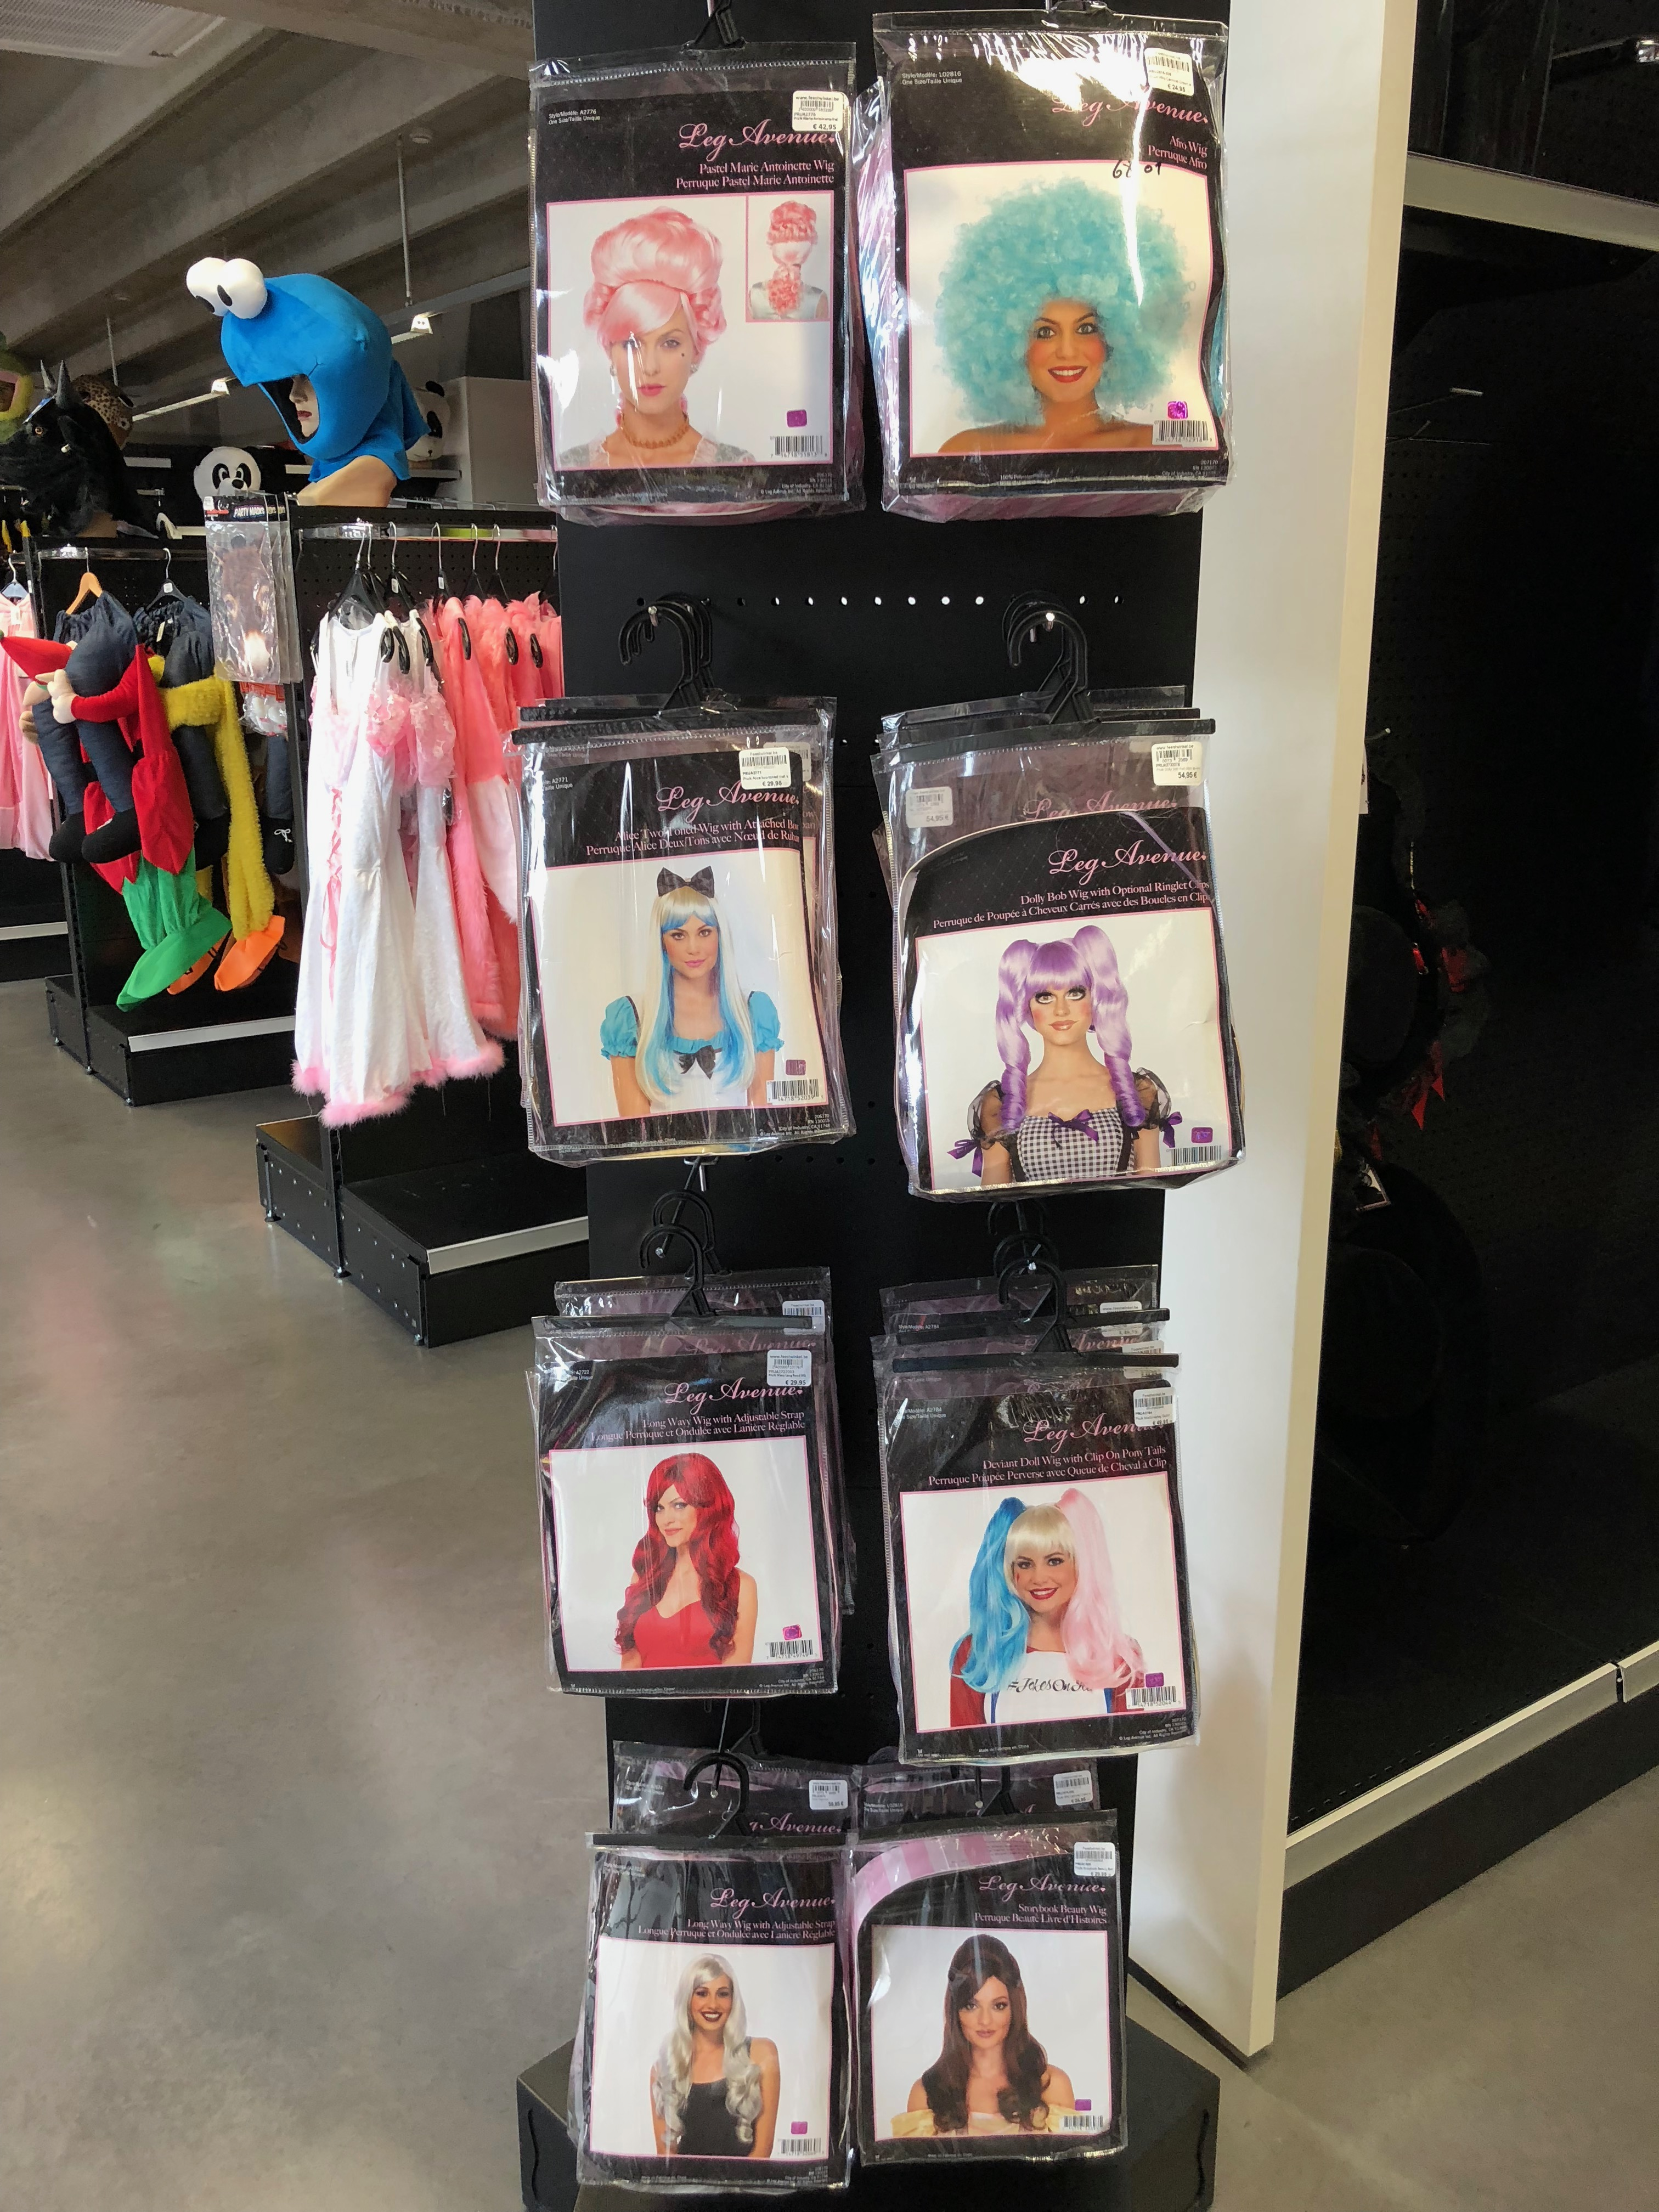
\includegraphics[width=0.4\textwidth]{img/rek.jpg}
    \caption{Producten die werden gebruikt voor de demoapplicatie}
    \label{fig:rek}
  \end{figure}

  \begin{figure}
    \centering
    \begin{subfigure}{.5\textwidth}
      \centering
      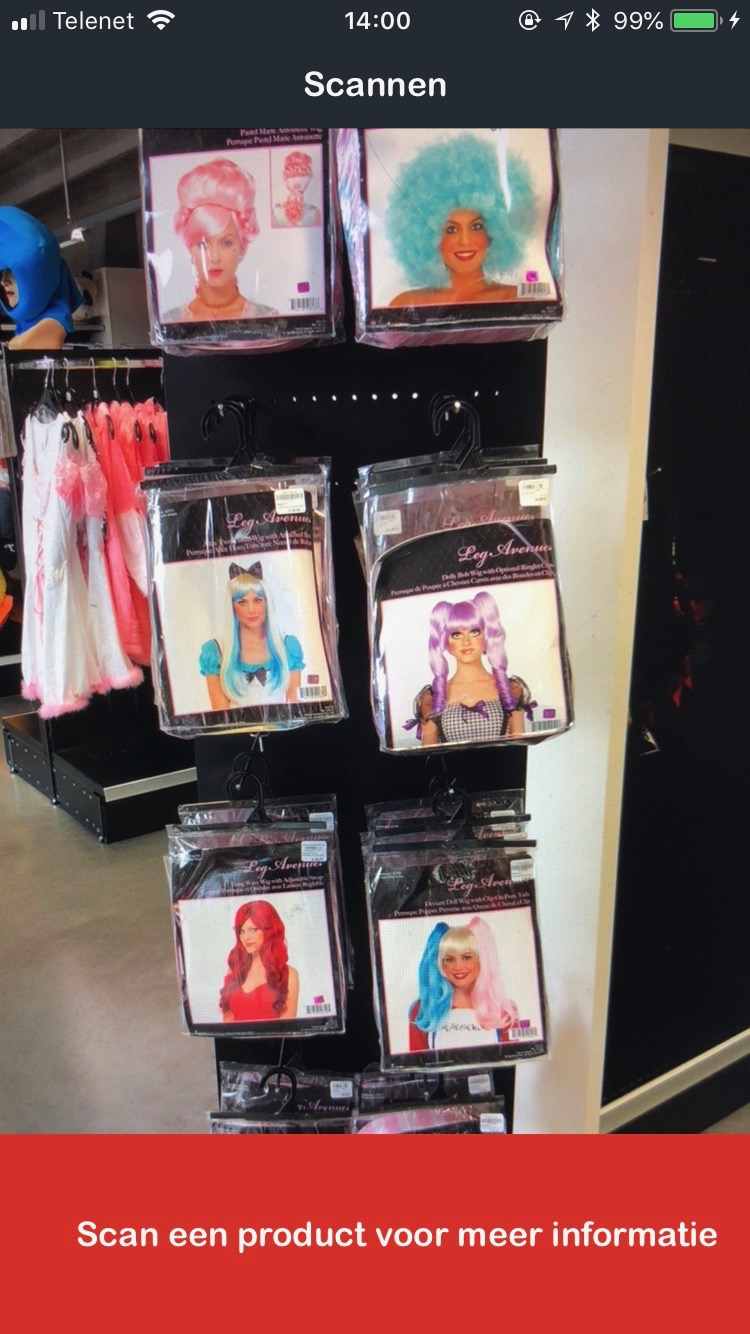
\includegraphics[width=.6\linewidth]{img/demoapp2.jpg}
      \caption{Het scherm voor het scannen}
      \label{fig:sub1}
    \end{subfigure}%
    \begin{subfigure}{.5\textwidth}
      \centering
      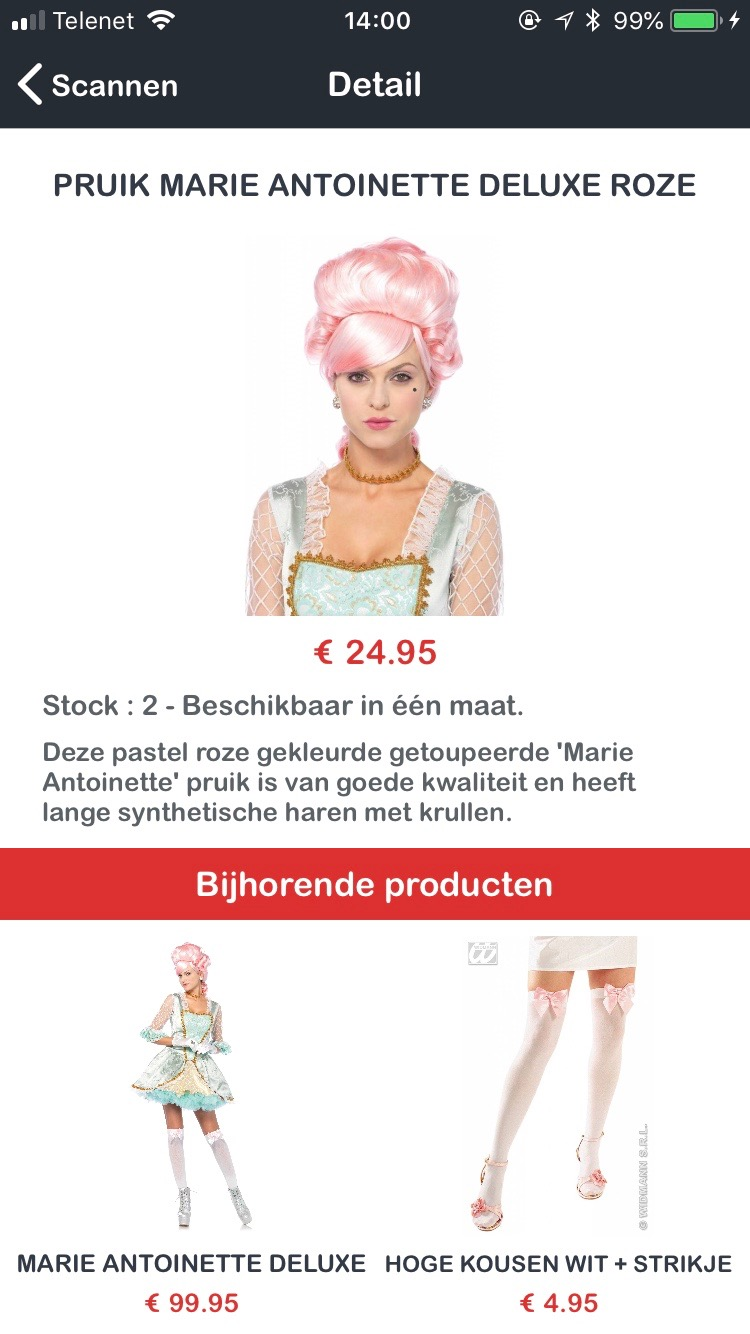
\includegraphics[width=.6\linewidth]{img/demoapp1.jpg}
      \caption{Productoverzicht na het scannen}
      \label{fig:sub2}
    \end{subfigure}
    \caption{Screenshots van de demoapplicatie}
    \label{fig:demoapp}
    \end{figure}

\section{Vragenlijst}
\label{sec:Vragenlijst}

Zoals eerder vermeld, werd aan klanten van de Feestwinkel gevraagd om de demoapplicatie uit te proberen. Na het uittesten werd er gevraagd om enkele vragen te beantwoorden. De vragenlijst bestond uit onderstaande vragen:
\begin{itemize}
    \item Zoals uzelf ervaren hebt, biedt de applicatie meer informatie over het product zoals het aantal stuks in voorraad en een omschrijving. Vindt u dat deze applicatie een meerwaarde biedt en zodus een extra hulpmiddel is voor u? 
    \item Naast informatie geeft de applicatie ook bijpassende of aan te raden producten weer wanneer een product scant. Zou u hierdoor geneigd zijn om sneller de betrokken producten te kopen, ook al had u niet gepland deze aan te kopen?
    \item Indien deze in de appstore verschijnt of er komt een applicatie voor een andere winkel of supermarkt, zou u desbetreffende applicatie installeren en effectief gaan gebruiken? 
\end{itemize}

  Op deze vragen waren de antwoordmogelijkheden ja of nee. Wanneer een klant op de laatste vraag ja antwoordde, dan werd er nog een gevraagd waarvoor hij de applicatie het meest zou gaan gebruiken. Onderstaande opsomming van mogelijke antwoorden werd aan de respondent voorgelegd:

\begin{itemize}
    \item De voorraad raadplegen
    \item De beschikbare maten controleren
    \item De bijpassende producten bekijken
    \item De aternatieve producten bekijken
\end{itemize}

De respondent kon hierbij meerdere antwoorden aankruisen.

\section{Resultaten}
\label{sec:Resultaten}

De resultaten van de vragenlijst uit voorgaand hoofdstuk boden antwoord op de laatste twee onderzoeksvragen. Van 30 dertig respondenten reageerden 28 met een ja op de eerste vraag. Meer dan 93\% vindt dus dat een applicatie die producten herkend uit een winkel en bovendien verdere informatie over dat herkend product geeft, een meerwaarde biedt aan desbetreffende winkel. 

Uit de resultaten was ook af te leiden dat het aanbieden van bijpassende producten invloed heeft op het koopgedrag van de gebruiker van de applicatie. 80\% wist positief te antwoorden op de tweede vraag. 

Hoewel 28 respondenten vindt dat een product herkennende applicatie een meerwaarde biedt een aan winkel, zou slechts 19 consumenten een gelijkaardige applicatie installeren op hun smartphone. De applicatie zou vooral gebruikt worden om de voorraad te raadplegen, de beschikbare maten controleren en om aanvullende producten te bekijken. In figuur \ref{fig:antwoordvraag} worden de antwoorden van de 19 respondenten procentueel weergegeven.

\begin{figure}[h!]
    \centering
        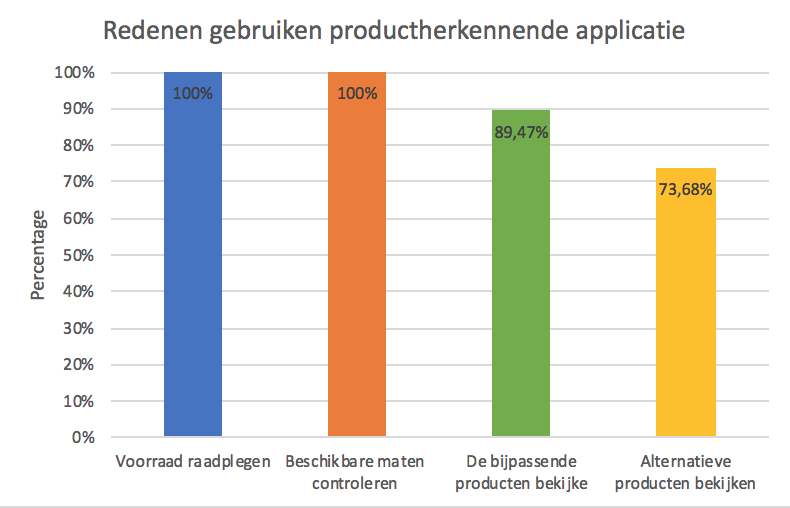
\includegraphics[width=0.8\textwidth]{img/antwoordenrespondenten.png}
    \caption{Grafische weergave van de antwoorden op de vierde vraag in percentage}
    \label{fig:antwoordvraag}
  \end{figure}

\section{Besluit}
\label{sec:Besluit}

De gebruikte vragenlijst is zodanig opgesteld dat ze antwoord biedt op de laatste twee onderzoeksvragen. Het is duidelijk dat een applicatie die producten herkend een meerwaarde biedt aan een fysieke winkel. Daarnaast kan het koopgedrag van de consument positief gestimuleerd worden door bijpassende producten aan te bieden. Niet elke bezoeker van een winkel zal bijhorende applicatie downloaden op hun smartphone. Sommige consumenten zijn namelijk te snel beïnvloedbaar en zijn zich daarvan bewust. Daarnaast zullen sommige klanten er geen behoefte aan hebben, of te weinig geheugen vrij hebben om een applicatie te downloaden die ze niet dagdagelijks gebruiken. Andere hebben nog steeds meer vertrouwen in personeel dan in een applicatie. 

